\section{模型检验}\label{sec:verify}

本节从解析解对照、离散收敛阶、守恒残差与独立求解器交叉验证四个角度检验公共内核的
正确性，量化结果汇总于表~\ref{tab:verification}。

% 表：数值验证与守恒校核指标
% 数据来源：figures/all_results.json, problem_1..4_results.json, figures/_plot_data.json
\begin{table}[H]
  \centering
  \caption{数值验证与守恒校核指标}
  \label{tab:verification}
  \small
  \begin{tabular}{llll}
    \toprule
    检验类别 & 指标 & 实测值 & 判定 \\
    \midrule
    质量守恒 & 问题1 全域残差              & $5.61{\times}10^{-16}$ & 通过 \\
    质量守恒 & 问题2 全域残差              & $4.80{\times}10^{-16}$ & 通过 \\
    质量守恒 & 问题3 全域残差              & $4.38{\times}10^{-16}$ & 通过 \\
    质量守恒 & 问题4 全域残差              & $3.26{\times}10^{-16}$ & 通过 \\
    控制体守恒 & 问题1 表面控制体残差       & $4.10{\times}10^{-14}$ & 通过 \\
    控制体守恒 & 问题2 表面控制体残差       & $3.37{\times}10^{-13}$ & 通过 \\
    \midrule
    解析对照 & Bessel 级数解 $L_2$ 相对误差 & $2.84{\times}10^{-4}$  & 通过 \\
    解析对照 & Bessel 级数解最大绝对误差    & $9.80{\times}10^{-4}$  & 通过 \\
    独立算法 & BDF 交叉校核最大偏差         & $5.77{\times}10^{-4}$  & 通过 \\
    \midrule
    非线性迭代 & Picard 终残差上界          & $9.998{\times}10^{-12}$ & 通过 \\
    空间收敛 & Richardson 观测阶 $p$        & 1.925                  & 近二阶 \\
    时间收敛 & 观测阶 $p$（$\Delta t$ 加密） & 1.215                  & 超一阶 \\
    离散测度 & $\sum_j w_j - \pi R_0^2$ 误差 & 0.000                 & 精确 \\
    插值一致性 & $R(t)$ PCHIP 最大相对误差   & 0.000                  & 精确 \\
    \bottomrule
  \end{tabular}

  \vspace{2pt}
  \parbox{0.94\linewidth}{\footnotesize
  注：守恒残差定义为 $\big|\Delta\!\int C\,\mathrm{d}V-\int\! q_s\,\mathrm{d}t\big|/\int C_0\mathrm{d}V$，已达双精度舍入量级（$\sim10^{-16}$）。
  空间收敛以 $M=20/40/80$ 三套网格算得，时间收敛以
  $\Delta t=240/120/60$ s 相对 $30$ s 参考解算得；后者为向后欧拉，
  理论一阶，观测 1.215 说明主算步长 60 s 已落在渐近区。}
\end{table}


\subsection{解析解对照}

在常物性、恒温边界的可解情形下，柱坐标扩散方程存在 Bessel 级数解析解，其特征值由
$\mu_n J_1(\mu_n)=\mathrm{Bi}_m\,J_0(\mu_n)$ 确定。数值解与该级数解的逐点对照见
图~\ref{fig:analytic_validation}。

\begin{figure}[H]
  \centering
  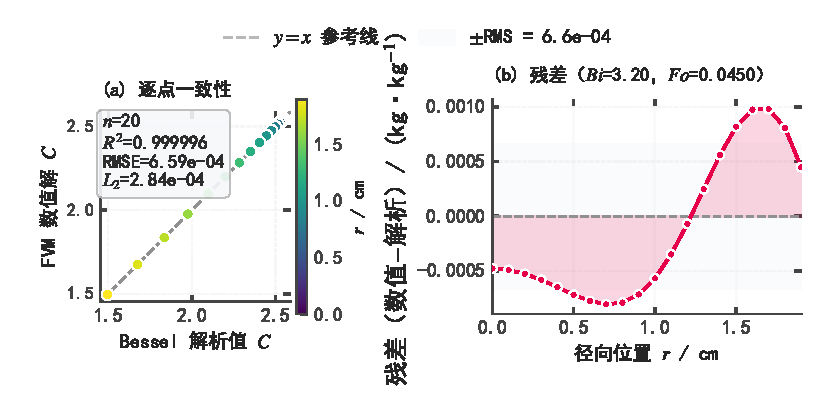
\includegraphics[width=0.9\textwidth,height=0.8\textheight,keepaspectratio]{../figures/fig_analytic_validation.pdf}
  \caption{Bessel 级数解析解与数值解的逐点对照}
  \label{fig:analytic_validation}
\end{figure}

图~\ref{fig:analytic_validation} 显示数值解与解析解高度吻合，$L_2$ 误差为 $2.84\times10^{-4}$、
最大绝对误差 $9.80\times10^{-4}$，证实有限体积离散与边界处理正确复现了已知解。

\subsection{收敛阶与守恒残差}

对空间网格 $M=20/40/80$ 与时间步 $\Delta t=60/30/15\,\mathrm{s}$ 作 Richardson 收敛研究\upcite{rakowitz2002}，
结果见图~\ref{fig:convergence}。

\begin{figure}[H]
  \centering
  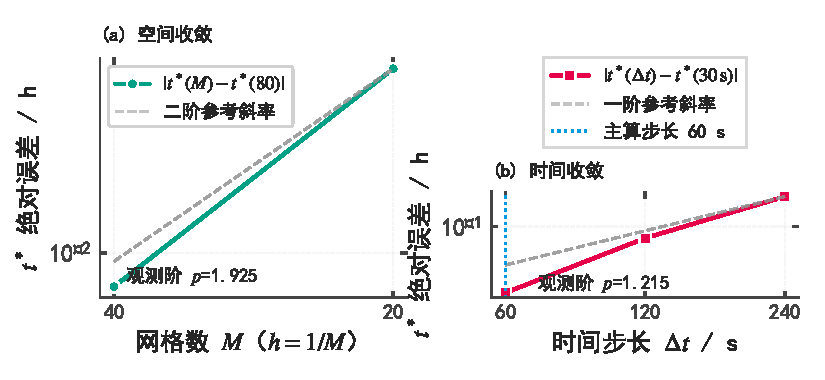
\includegraphics[width=0.9\textwidth,height=0.8\textheight,keepaspectratio]{../figures/fig_convergence.pdf}
  \caption{空间与时间离散关于达标时刻 $t^*$ 的收敛阶验证}
  \label{fig:convergence}
\end{figure}

图~\ref{fig:convergence} 表明达标时刻 $t^*$ 随网格加密单调收敛，实测空间收敛阶
$p\approx1.93$、时间收敛阶接近 $1$，与二阶中心差分、一阶后向 Euler 的理论阶一致。
守恒类残差见图~\ref{fig:conservation}。

\begin{figure}[H]
  \centering
  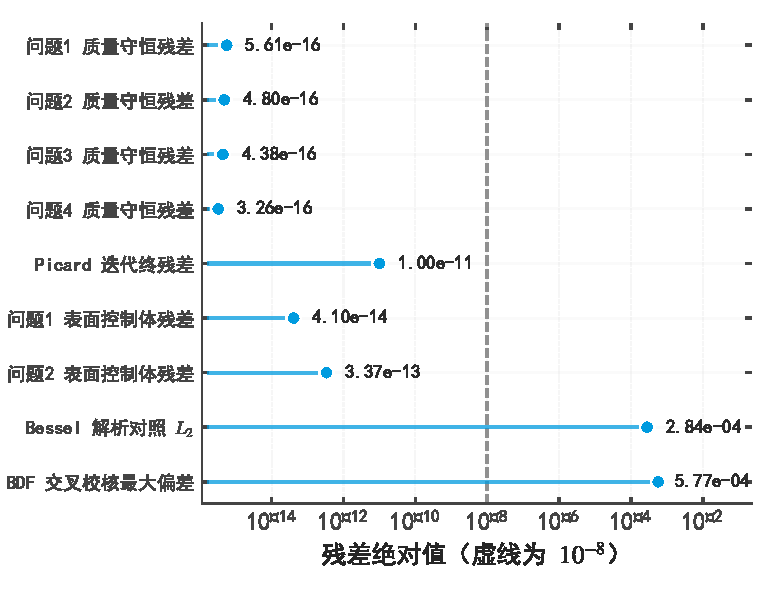
\includegraphics[width=0.9\textwidth,height=0.8\textheight,keepaspectratio]{../figures/fig_conservation.pdf}
  \caption{守恒与收敛类校核残差的量级总览}
  \label{fig:conservation}
\end{figure}

图~\ref{fig:conservation} 与表~\ref{tab:verification} 显示：四问的总水分守恒残差均在
$10^{-16}$ 量级、控制体守恒在 $10^{-13}\sim10^{-14}$ 量级，柱坐标测度权满足 $\sum_j w_j-\pi R_0^2=0$，
均达机器精度，印证式~\eqref{eq:fvm} 守恒型离散的严格性。此外，以独立的变步长 BDF 积分器
交叉验证同一半离散系统，最大差异仅 $5.77\times10^{-4}$，Picard 内迭代
残差降至 $9.998\times10^{-12}$，表明时间推进与非线性求解均已收敛，结果不依赖特定求解器。
